\documentclass[12 pt]{article}
\usepackage[utf8]{inputenc}
\usepackage{matlab-prettifier}
\usepackage[portuguese]{babel}
\usepackage{indentfirst}
\usepackage{graphicx}
\usepackage{float}
\usepackage{subcaption}
\usepackage[font=small,labelfont=bf]{caption}
\definecolor{mygreen}{RGB}{28,172,0} % color values Red, Green, Blue
\definecolor{myyellow}{rgb}{1.0, 1.0, 0.8}
\usepackage{mathtools}
\usepackage{multirow}
\usepackage{comment}
\usepackage{xcolor}
\usepackage{colortbl}
\usepackage[normalem]{ulem}               % to striketrhourhg text
\usepackage{amsmath}
\usepackage{amsfonts}
\usepackage{hyperref}
\newcommand\redout{\bgroup\markoverwith
{\textcolor{red}{\rule[0.5ex]{2pt}{0.8pt}}}\ULon}
\renewcommand{\lstlistingname}{Código}% Listing -> Algorithm
\renewcommand{\lstlistlistingname}{Lista de \lstlistingname s}% List of Listings -> List of Algorithms

\usepackage[top=3cm,left=2cm,bottom=2cm, right=2cm]{geometry}
\usepackage{tikz}
\usetikzlibrary{decorations.pathreplacing}


% Configuração para destacar a sintaxe do Python
\lstset{ 
    language=Python,                     % A linguagem do código
    backgroundcolor=\color{myyellow}, % A cor do fundo 
    basicstyle=\ttfamily\footnotesize,   % O estilo do texto básico
    keywordstyle=\color{blue},           % Cor das palavras-chave
    stringstyle=\color{red},             % Cor das strings
    commentstyle=\color{mygreen},          % Cor dos comentários
    numbers=left,                        % Números das linhas à esquerda
    numberstyle=\tiny\color{gray},       % Estilo dos números das linhas
    stepnumber=1,                        % Número de linhas entre os números das linhas
    frame=single,                        % Moldura ao redor do código
    breaklines=true,                     % Quebra automática das linhas longas
    captionpos=t,                        % Posição da legenda
    showstringspaces=false               % Não mostra espaços em branco nas strings
    extendedchars=true,
    literate={º}{{${ }^{\underline{o}}$}}1 {á}{{\'a}}1 {à}{{\`a}}1 {ã}{{\~a}}1 {é}{{\'e}}1 {É}{{\'E}}1 {ê}{{\^e}}1 {ë}{{\"e}}1 {í}{{\'i}}1 {ç}{{\c{c}}}1 {Ç}{{\c{C}}}1 {õ}{{\~o}}1 {ó}{{\'o}}1 {ô}{{\^o}}1 {ú}{{\'u}}1 {â}{{\^a}}1 {~}{{$\sim$}}1
}


\title{%
\textbf{\huge Universidade Federal do Rio de Janeiro} \par
\textbf{\LARGE Instituto Alberto Luiz Coimbra de Pós-Graduação e Pesquisa de Engenharia} \par

\includegraphics[width=8cm]{COPPE UFRJ.png} \par
\textbf{Programa de Engenharia de Sistemas e Computação} \par
\large
CPS769 - Introdução à Inteligência Artificial e Aprendizagem Generativa \newline \par
\small
Prof. Dr. Edmundo de Souza e Silva (PESC/COPPE/UFRJ)\par 
Profa. Dra. Rosa M. Leão (PESC/COPPE/UFRJ)\par 
Participação Especial: Gaspare Bruno (Diretor Inovação, ANLIX) \par

\vspace{1\baselineskip}
\Large
\textbf{\textit{Lista de Exercícios 1a
}}
}

\author{Luiz Henrique Souza Caldas\\email: lhscaldas@cos.ufrj.br}

\date{\today}

\begin{document}
\maketitle

\section*{Questão 1}

Esse exemplo simples é para auxiliar a discussão do artigo “Serial Order A Parallel Distributed Processing Approach” que todos já devem ter lido. O objetivo é prever um padrão de figura, por exemplo um quadrado, usando uma Rede Neural Recorrente (RNN). Fornecemos o código em Python de um exemplo de geração do padrão 2-D de quadrados e treinamento de uma RNN para prever a sequência cíclica [0, 25, 0, 25], [0, 75, 0, 25], [0, 75, 0, 75], [0, 25, 0, 75], [0, 25, 0, 25].

\begin{enumerate}
    \item Entenda o código e explique qual a RNN que ele modela (faça o desenho). Explique a parte do código que define a RNN.
    
    \textbf{Resposta:} \par

    O código pode ser explicado dividindo-o em 6 partes:
    \begin{enumerate}
        \item Definição do caminho quadrado: O código define um conjunto de coordenadas que formam um caminho quadrado na variável \textit{square\_path}.
        \begin{lstlisting}[language=Python]
square_path = np.array([
    [0.25, 0.25],
    [0.75, 0.25],
    [0.75, 0.75],
    [0.25, 0.75],
    [0.25, 0.25]
])
        \end{lstlisting}
        \item Geração dos dados de treinamento: O caminho quadrado é repetido várias vezes para formar os dados de treinamento.
        \begin{lstlisting}[language=Python]
num_repeats = 4
data = np.tile(square_path, (num_repeats, 1))
x_train = data[:-1].reshape(-1, 1, 2)
y_train = data[1:].reshape(-1, 2)
        \end{lstlisting}
        \item Definição e compilação do modelo RNN: O modelo RNN é definido usando uma camada LSTM (\textit{long short-term memory}) seguida de uma camada densa e depois é compilado configurando o algoritmo ADAM como otimizador e o Erro Médio Quadrático como função de perda.
        \begin{lstlisting}[language=Python]
model = models.Sequential([
    layers.LSTM(50, activation='relu', input_shape=(num_repeats, 2)),
    layers.Dense(2)
])
model.compile(optimizer='adam', loss='mse')            
        \end{lstlisting}

        \begin{figure}[H]
            \centering
            \begin{tikzpicture}[
                neuron/.style={draw, circle, minimum size=2cm, align=center},
                lstm/.style={draw, rectangle, minimum width=2cm, minimum height=1cm, align=center},
                ->, >=stealth
            ]
        
            % Nodes
            \node[neuron] (input1) at (0, 1.1) {Input 1};
            \node[neuron] (input2) at (0, -1.1) {Input 2};
            \node[lstm] (lstm) at (4, 0) {Camada LSTM \\ (50 neurônios)};
            \node[neuron] (output1) at (8, 1.1) {Output 1};
            \node[neuron] (output2) at (8, -1.1) {Output 2};
        
            % Brace for Dense Layer
            \draw [decorate,decoration={brace,amplitude=10pt,mirror,raise=5pt}] (9,-1.5) -- (9,1.5);
            
            % Text for Dense Layer
            \node at (11, 0) {Camada densa};
        
            % Edges
            \draw [->] (input1) -- (lstm);
            \draw [->] (input2) -- (lstm);
            \draw [->] (lstm) -- (output1);
            \draw [->] (lstm) -- (output2);
        
            \end{tikzpicture}
            \caption{Diagrama de uma Rede Neural Recorrente (RNN) com dois neurônios de entrada e dois neurônios de saída (camada densa) e uma camada LSTM modelada no código fornecido.}
            \label{fig:rnn_diagram}
        \end{figure}

        \item Treinamento do modelo: O modelo é treinado com os dados gerados, utilizando inicialmente 300 épocas.
        \begin{lstlisting}[language=Python]
model.fit(x_train, y_train, epochs=300, verbose=0)
        \end{lstlisting}
        \item Geração das previsões: As previsões são geradas.
        \begin{lstlisting}[language=Python]
predictions = model.predict(x_train[:5])
        \end{lstlisting}
        \item  Plotagem dos resultados: As previsões são plotadas e comparadas com o caminho original.
        \begin{lstlisting}[language=Python]
plt.plot(data[:, 0], data[:, 1], label='Original Path', linestyle='dashed', color='gray')
plt.plot(predictions[:, 0], predictions[:, 1], label='Predicted Path', color='blue')
plt.scatter(square_path[:, 0], square_path[:, 1], color='red')
plt.legend()
plt.show()
        \end{lstlisting}
    \end{enumerate}
    \item Treine a rede. Aprenda como fazer, e explique.
   
    \textbf{Resposta:} \par

    Como dito no passo (d) do item anterior, o treinamento é ralizado utilizando a função "fit" do modelo. Utilizando a configuração inicial, com 300 épocas, o treinamento demorou cerca de 11 segundos.


    \item Faça a previsão de algumas trajetórias, quando o ponto inicial varia. O que você conclui?
   
    \textbf{Resposta:} \par

    Foi feita a previsão para o ponto inicial original do código dado, $(x_1=0.25$ e $x_2=0.25)$ e depois foram testados os outros vértices do quadrado. Para isso foi implementada a função \textit{plot\_predictions\_with\_varied\_initial\_points} (código no final do relatório), na qual os pontos são previstos em sequência, sendo a previsão anterior a entrada da próxima previsão, somando um total de 4 previsões para cada ponto inicial. O resultado pode ser observado na figura abaixo.

    \begin{figure}[H]
        \caption{Previsão para diferentes pontos iniciais}
           \centering
           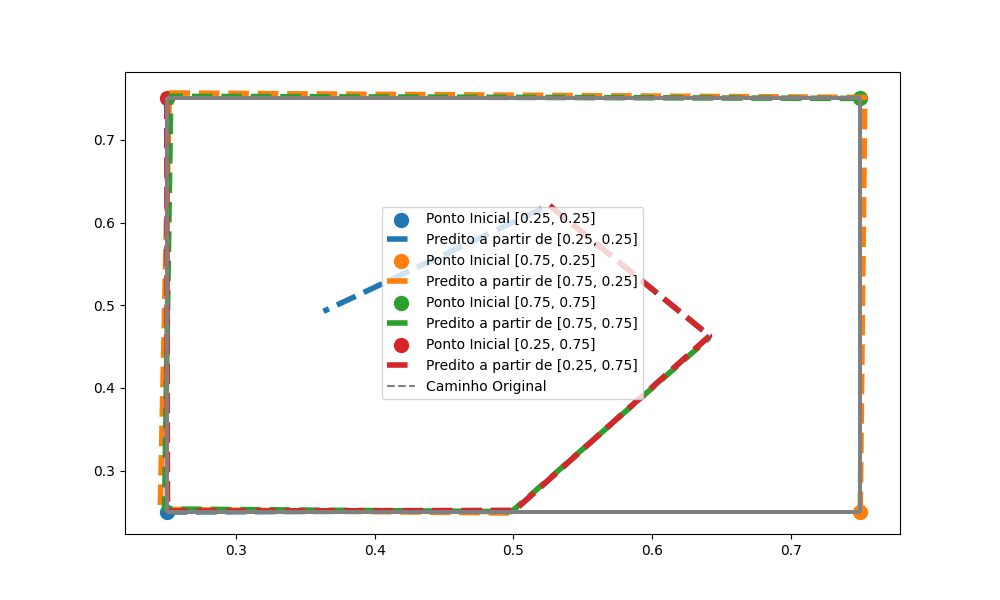
\includegraphics[height=8cm]{fig/Item_3.png}
    \end{figure}
    
    Todas as previsões divergem do caminho original no ponto $(x_1=0.50$ e $x_2=0.25)$, o que indica uma provavél incompatibilidade do modelo para prever esse caminho, uma vez que foram testadas diversas variações de número de épocas e de repetições do caminho original no treinamento.

    \item Modifique a RNN usada e observe o que acontece.

    \textbf{Resposta:} \par

    Para este teste, o ponto inicial foi retornado para a configuração original $(x_1=0.25$ e $x_2=0.25)$ e foram testadas diferentes combinações de épocas e número de repetições.

    \begin{table}[H]
        \centering
        \caption{Resultados das modificações}
        \begin{tabular}{|c|c|c|c|}
            \hline
            Nº Repetições & Épocas & Tempo Treinamento (s) & Tempo Total (s) \\
            \hline
            4 & 300 & 12 & 12.2 \\
            \hline
            40 & 300 & 13.5 & 13.7 \\
            \hline
            400 & 300 & 26.4 & 26.6 \\
            \hline
            40 & 600 & 19.6 & 19.8 \\
            \hline
            40 & 900 & 29.2 & 29.1 \\
            \hline
        \end{tabular}
    \end{table}

    Pela tabela 1 é possível observar o aumento do tempo de execução, mais específicamente do tempo de treinamento, tanto com o aumento do número de repetições quanto com o aumento do número de épocas. Os resultados das previsões podem ser visualizados nas figuras abaixo.
    

    \begin{figure}[H]
        \caption{Previsão para 4 repetições e 300 épocas}
           \centering
           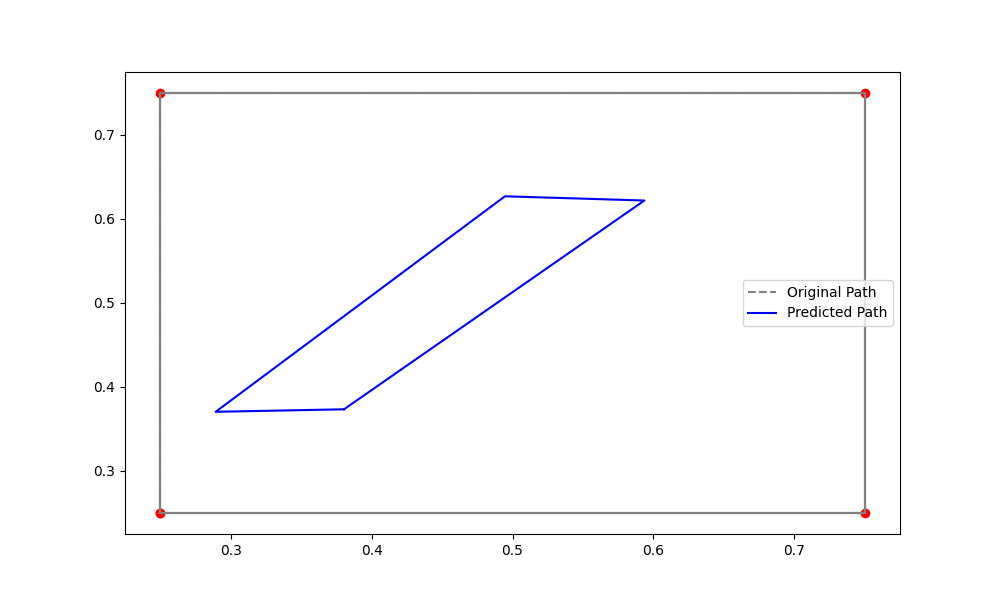
\includegraphics[height=8cm]{fig/Item_4_4_300.png}
    \end{figure}

    \begin{figure}[H]
        \caption{Previsão para 40 repetições e 300 épocas}
           \centering
           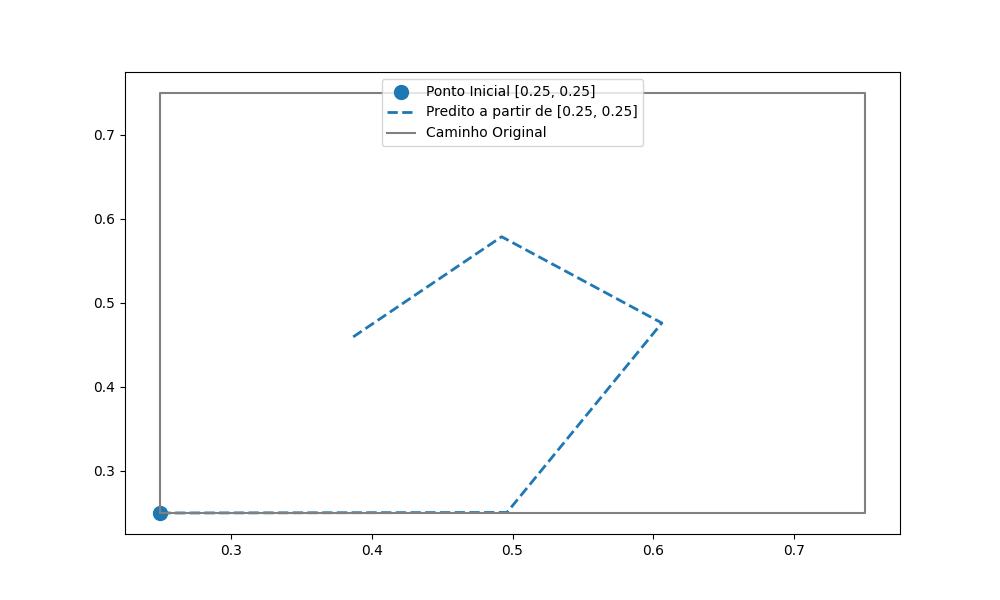
\includegraphics[height=8cm]{fig/Item_4_40_300.png}
    \end{figure}

    \begin{figure}[H]
        \caption{Previsão para 400 repetições e 300 épocas}
           \centering
           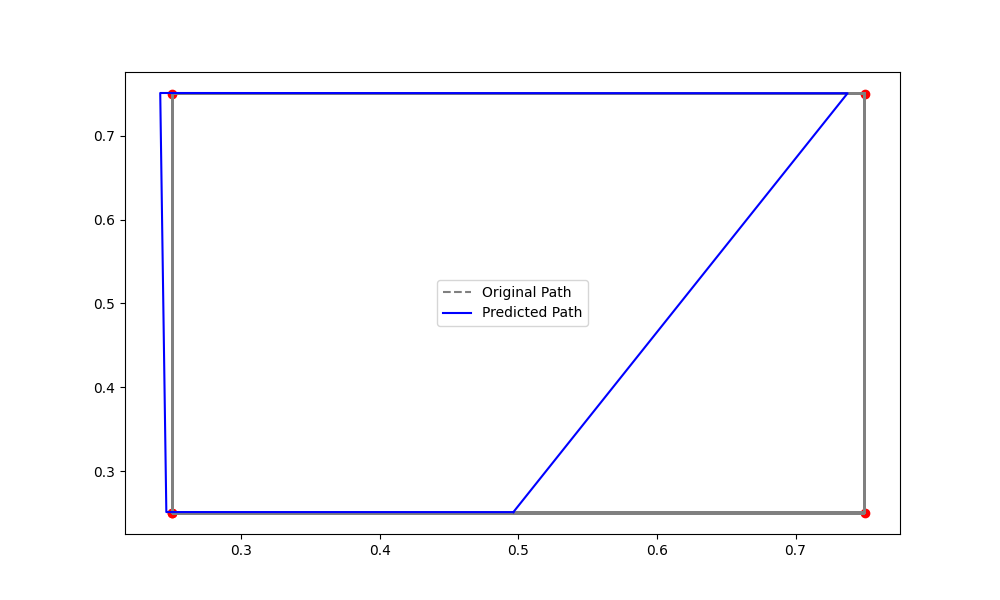
\includegraphics[height=8cm]{fig/Item_4_400_300.png}
    \end{figure}

    \begin{figure}[H]
        \caption{Previsão para 40 repetições e 600 épocas}
           \centering
           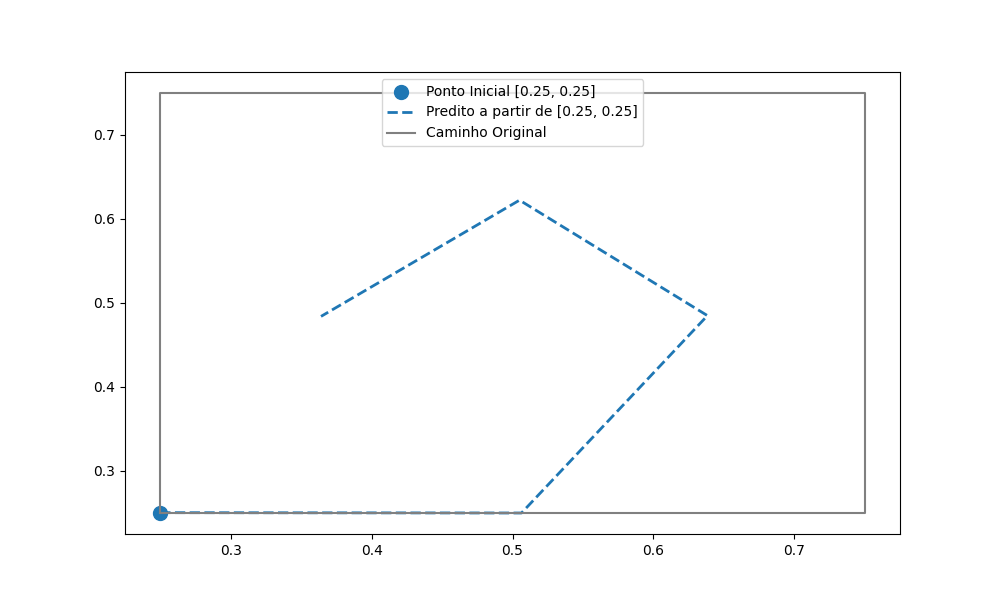
\includegraphics[height=8cm]{fig/Item_4_40_600.png}
    \end{figure}


    \begin{figure}[H]
        \caption{Previsão para 40 repetições e 900 épocas}
           \centering
           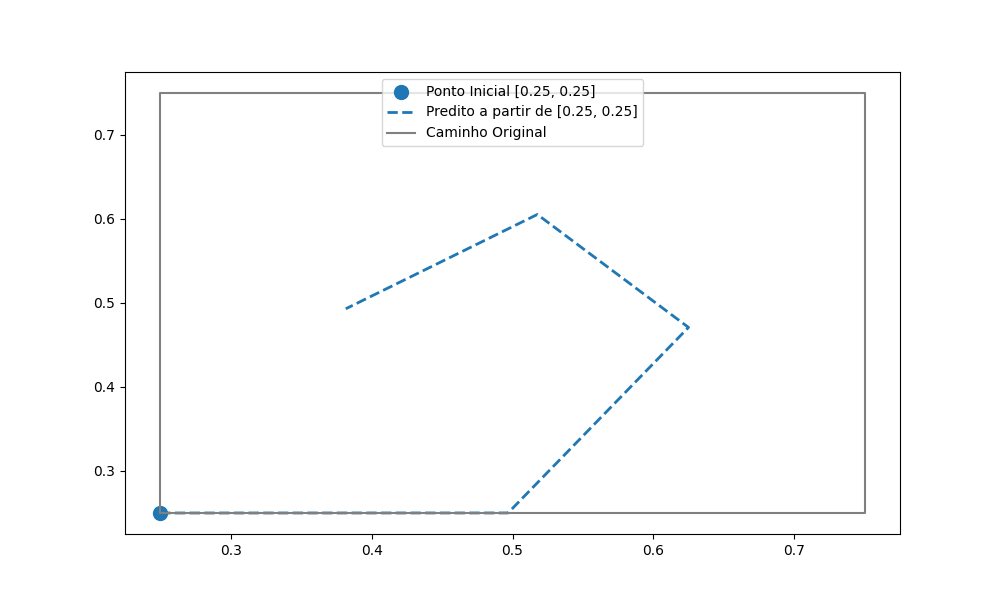
\includegraphics[height=8cm]{fig/Item_4_40_900.png}
    \end{figure}
    
    Pelas figuras foi possível observar que o impacto do aumento do número de repetições na precisão da previsão foi muito maior que o impacto do aumento do número de épocas, o que demonstra a importância do tamanho do dataset de treinamento para o resultado de suas previsões.

    \item Quais os pontos principais que você concluiu do artigo “Serial Order A Parallel Distributed Processing Approach”?
        
    \textbf{Resposta:} \par

    A teoria de Michael I. Jordan sobre ordem serial em sequências de ações usa redes neurais para entender e reproduzir a ordem das ações ao longo do tempo. Essas redes mantêm uma "memória" do que já aconteceu, usando conexões que alimentam as saídas de volta para as entradas, ajudando a lembrar das ações passadas. A rede aprende ajustando seus parâmetros para reduzir erros entre o que foi previsto e o que realmente aconteceu.

    Isso faz com que a rede consiga generalizar a partir de sequências aprendidas e continuar funcionando bem, mesmo com pequenas perturbações. Essencialmente, a rede se torna uma memória dinâmica que pode voltar às suas trajetórias aprendidas, garantindo que as sequências de ações sejam produzidas corretamente, mesmo começando de pontos diferentes.

    \item Qual a differença da RNN usada no código em relação ao artigo “Serial Order A Parallel Distributed Processing Approach”?
        
    \textbf{Resposta:} \par

    No artigo, a rede é composta por unidades de plano, estado e saída, com conexões recorrentes que definem a função de próximo estado, e enfatiza a capacidade de aprender e generalizar trajetórias no espaço de estado. Em contraste, a RNN do código usa uma arquitetura LSTM simples, que captura dependências temporais através de sua memória interna, sem distinções explícitas entre plano e estado. A abordagem de Jordan foca em representações distribuídas e paralelismo, enquanto a RNN do código adota técnicas convencionais de redes neurais recorrentes.

    \item Inclua, nos dados de treino uma figura de uma espiral quadrada, e experimente o que a rede aprendeu.
        
    \textbf{Resposta:} \par

    Para gerar o caminho em espiral foi implementada a função \textit{generate\_spiral\_square} (código no final do relatório), a qual gera uma lista no mesmo formato da \textit{square\_path} fornecida, porém com os pontos formando uma espiral quadrada. O resultado da previsão pode ser observado na figura abaixo.

\end{enumerate}

\section*{Código}

O código abaixo encontra-se no repositório \href{https://github.com/lhscaldas/cps769-ai-gen}{https://github.com/lhscaldas/cps769-ai-gen}, bem como o arquivo LaTex com o relatório.


\lstinputlisting[language=Python,caption=código fornecido completo com algumas modificações]{Lista_1a_v2.py}

\end{document}